\documentclass[a4paper,12pt]{book}
\usepackage{ngerman}
\usepackage{times}
\usepackage{amsmath}
\usepackage{amssymb}
\usepackage{amsfonts}
\usepackage{amsthm}
\usepackage{graphicx}
\usepackage{fancyhdr}
\usepackage{textcomp}
\usepackage[all]{xy}
\usepackage{txfonts}
\usepackage{alltt}
\usepackage{verbatim}
\usepackage{paralist}
\usepackage{makeidx}
\usepackage{array}
\usepackage{hyperref}
\usepackage{tikz}
\usetikzlibrary{arrows,shapes,snakes}
\makeindex



\begin{document}
\pagestyle{fancy}
%\lhead{Optimierung}
\frontmatter
\newcommand\HRule{\noindent\rule{\linewidth}{1.5pt}}

\begin{titlepage}
\vspace*{\stretch{1}}
\HRule
\vspace*{10pt}
\begin{flushright}
{\Huge
Simplex Algorithmus f�r nichtlineare Optimierungsprobleme}
\end{flushright}
\HRule
\begin{flushright}
\vspace{30pt}
\LARGE
Selina Malacarne, Raphael Nestler
\end{flushright}
\vspace*{\stretch{2}}
\begin{center}
Hochschule f"ur Technik, Rapperswil, 2012
\end{center}
\end{titlepage}

\hypersetup{
    colorlinks=true,
    linktoc=all,
    linkcolor=blue
}

\setcounter{tocdepth}{2}
\tableofcontents
\mainmatter

\chapter{Simplex-Downhill}
\chapter{Einleitung}
Der Simplex-Downhill-Algorithmus ist eine Methode zur Optimierung nicht-linearer n-dimensionaler Funktionen. \\
Dieses Verfahren wurde von den britischen Statistikern John Nelder und Roger Mead entwickelt und gilt vor allem bei Problemen mit 
geringem rechnerischen Aufwand als die schnellstmögliche Methode. 

%--------------------------------------------------------------------------------------------------------------------------------------------
%General Stuff
%--------------------------------------------------------------------------------------------------------------------------------------------
\section{Simplex}
Ein Simplex ist ein Begriff, welcher aus der Geometrie stammt. Er beschreibt ein n-dimensionales Polytop. Wobei ein Polytop die Bezeichnung für ein verallgemeinertes Polygon ist, sprich ein verallgemeinertes Vieleck. 
Hier einige vorstellbare Beispiele zum Simplex:\\
 
\begin{tabular}{c|l}
Dimension & Geometrische Form\\
\hline
$n=0$ & Punkt\\
$n=1$ & Strecke\\
$n=2$ & Dreieck\\
$n=3$ & Tetraeder
\end{tabular} 

Aus der Tabelle wird ersichtlich, dass jeder n-dimensionale Simplex genau n+1 Ecken hat.

Im Downhilh-Simplex-Verfahren wird der Simplex benötigt, um die optimalen Parameterwerte zu finden. Man kann es sich so vorstellen, dass der Simplex im n-dimensionalen Parameterraum aufgespannt wird und dann für jeden Punkt des Simplex die Fehlerfunktion berechnet wird.

Der schlechteste dieser Punkte wird dann mittels gewisse "Taktiken" ersetzt und dies wird solange fort geführt, bis das Ergebnis erreicht worden ist. 

%--------------------------------------------------------------------------------------------------------------------------------------------

\section{Modifikationen des Simplex}
Die Möglichkeiten den Simplex soweit zu verändern, dass er den optimalen Punkt findet, sind begrenzt.

Es gibt einige Modifikationen, welche man auf den Simplex anwenden kann. Die Darstellungen beziehen sich hierbei auf einen Simplex der zweiten Dimension (Dreieck), natürlich gelten diese Modifikationen auch für den n-dimensionalen Simplex.

\begin{figure}[h]
	\centering
	
\usetikzlibrary{arrows}

\definecolor{uuuuuu}{rgb}{0.27,0.27,0.27}
\definecolor{zzttqq}{rgb}{0.6,0.2,0}
\definecolor{qqqqff}{rgb}{0,0,1}
\begin{tikzpicture}[line cap=round,line join=round,>=triangle 45,x=1.0cm,y=1.0cm]
\clip(5.07,1.09) rectangle (11.72,4.37);
\fill[color=zzttqq,fill=zzttqq,fill opacity=0.1] (5.74,2.92) -- (10.36,3.74) -- (11,1.52) -- cycle;
\draw [color=zzttqq] (5.74,2.92)-- (10.36,3.74);
\draw [color=zzttqq] (10.36,3.74)-- (11,1.52);
\draw [color=zzttqq] (11,1.52)-- (5.74,2.92);
\begin{scriptsize}
\fill [color=qqqqff] (5.74,2.92) circle (1.5pt);
\draw[color=qqqqff] (5.76,3.15) node {$x_{min}$};
\fill [color=qqqqff] (10.36,3.74) circle (1.5pt);
\draw[color=qqqqff] (10.73,3.9) node {$x_{max}$};
\fill [color=qqqqff] (11,1.52) circle (1.5pt);
\draw[color=qqqqff] (11.17,1.68) node {$x_3$};
\fill [color=uuuuuu] (8.05,3.33) circle (1.5pt);
\draw[color=uuuuuu] (8.46,3.56) node {$x_{1neu}$};
\fill [color=uuuuuu] (8.37,2.22) circle (1.5pt);
\draw[color=uuuuuu] (8.79,2.39) node {$x_{3neu}$};
\fill [color=uuuuuu] (9.03,2.73) circle (1.5pt);
\draw[color=uuuuuu] (9.28,2.67) node {$x_m$};
\end{scriptsize}
\end{tikzpicture}
%
  	\caption{bla}%
	\label{fig:Dreiecke}%
\end{figure}



\section{Der Algorithmus}

\subsection{Hauptablauf Algorithmus}
Zu Beginn wird ein Simplex gebildet, indem f"ur jede Ecke i des Simplex ein $x_i$ ausgew"ahlt wird. 
Mit den gew"ahlten $x_i$ werden nun die dazu geh"origen $y_i$ der Zielfunktion ausgerechnet. \\
Aus den erhaltenen Funktionswerten wird der beste $y_{min}$ sowie der schlechteste $y_{max}$ betrachtet. Wenn der beste Wert gut genug ist, dann ist der Algorithmus schon fertig, bevor er eigentlich begonnen hat. Es ist nat"urlich eher Zufall, wenn man gleich bei der ersten Wahl des Simplex das Minima trifft, meistens hat man es nicht getroffen und muss nun auf Grund des gew"ahlten Simplex ein neues Simplex bilden. 

\resizebox{1\textwidth}{!}{
\providecommand{\highlight}{white}
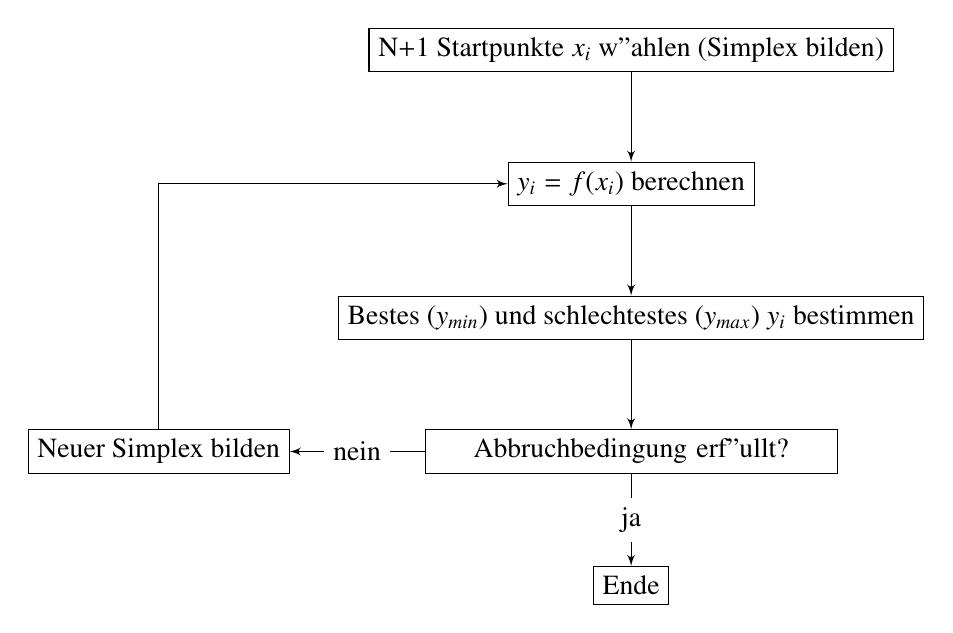
\begin{tikzpicture}[node distance = 1.7cm,every node/.style={rectangle,fill=white},
  block/.style={draw,align=center},
  highlight/.style={draw,fill=\highlight},
  line/.style = {draw,-latex'}
]

\node (start) [block] {N+1 Startpunkte $x_i$ w"ahlen (Simplex bilden)};

\node (a1) [block, below of=start] { $y_i = f(x_i)$ berechnen};

\node (a2) [block, below of=a1] { Bestes ($y_{min}$) und schlechtestes ($y_{max}$) $y_i$ bestimmen};

\node (a3) [block, below of=a2,text width=5cm]{Abbruchbedingung erf"ullt?};

\node (ende) [block, below of=a3] {Ende};

\node (a4) [highlight, left of=a3, node distance=6cm] {Neuer Simplex bilden};



\path[line] (start) -- (a1);
\path[line] (a1) -> (a2);
\path[line] (a2) -> (a3);

\path[line] (a3) -> node{ja} (ende);
\path[line] (a3) -> node{nein} (a4);

\path[line] (a4)  |-  (a1.west);

\end{tikzpicture}
}


\subsection{Auswahlverfahren neues Simplex}
Das Auswahlverfahren des neuen Simplex unterliegt eine Reihe von Entscheidungen auf Grund der gegebenen Eckpunkte sowie deren Funktionswerte. Auf Seite XXX findet man diesen Entscheidungsbaum.\\
Wenn man das Diagramm etwas genauer betrachtet, f"allt einem auf, dass zu Beginn das Simplex ziemlich grob behandelt wird, indem man erst einmal durch Reflexion versucht, weg vom schlechtesten Punkt zu kommen. War diese Entscheidung erfolgreich wird auch noch gleich in die neue Richtung gestreckt, um das Simplex in die vermeintlich richtige Richtung zu treiben. \\
Erst wenn diese Methode nicht funktioniert hat, wird etwas detaillierter auf das Simplex und seine Position eingegangen, indem man beispielsweise schaut, ob der reflektierte Funktionswert zumindest besser ist als der zweitschlechteste. \\
Methoden wie die Kontraktion oder auch die Komprimierung sind dann schliesslich eher Feineinstellungen, man versucht etwas n"aher zum Schwerpunkt zu r"ucken, um zu schauen, wie sich die neuen Eckpunkte in der Zielfunktion verhalten.\\
Das ganze ist nat"urlich sehr abh"angig von dem zu Beginn gew"ahlten Simplex. Der Algorithmus findet - bis auf wenige Ausnahmen - immer ein Minima. Wenn er jedoch st"andig in ein lokales Minima f"allt, muss man sich vielleicht "uberlegeben die Startbedingungen zu "andern, indem man das Simplex beispielsweise "uber ein gr"osseres Gebiet aufspannt.\\
\usetikzlibrary{shapes}
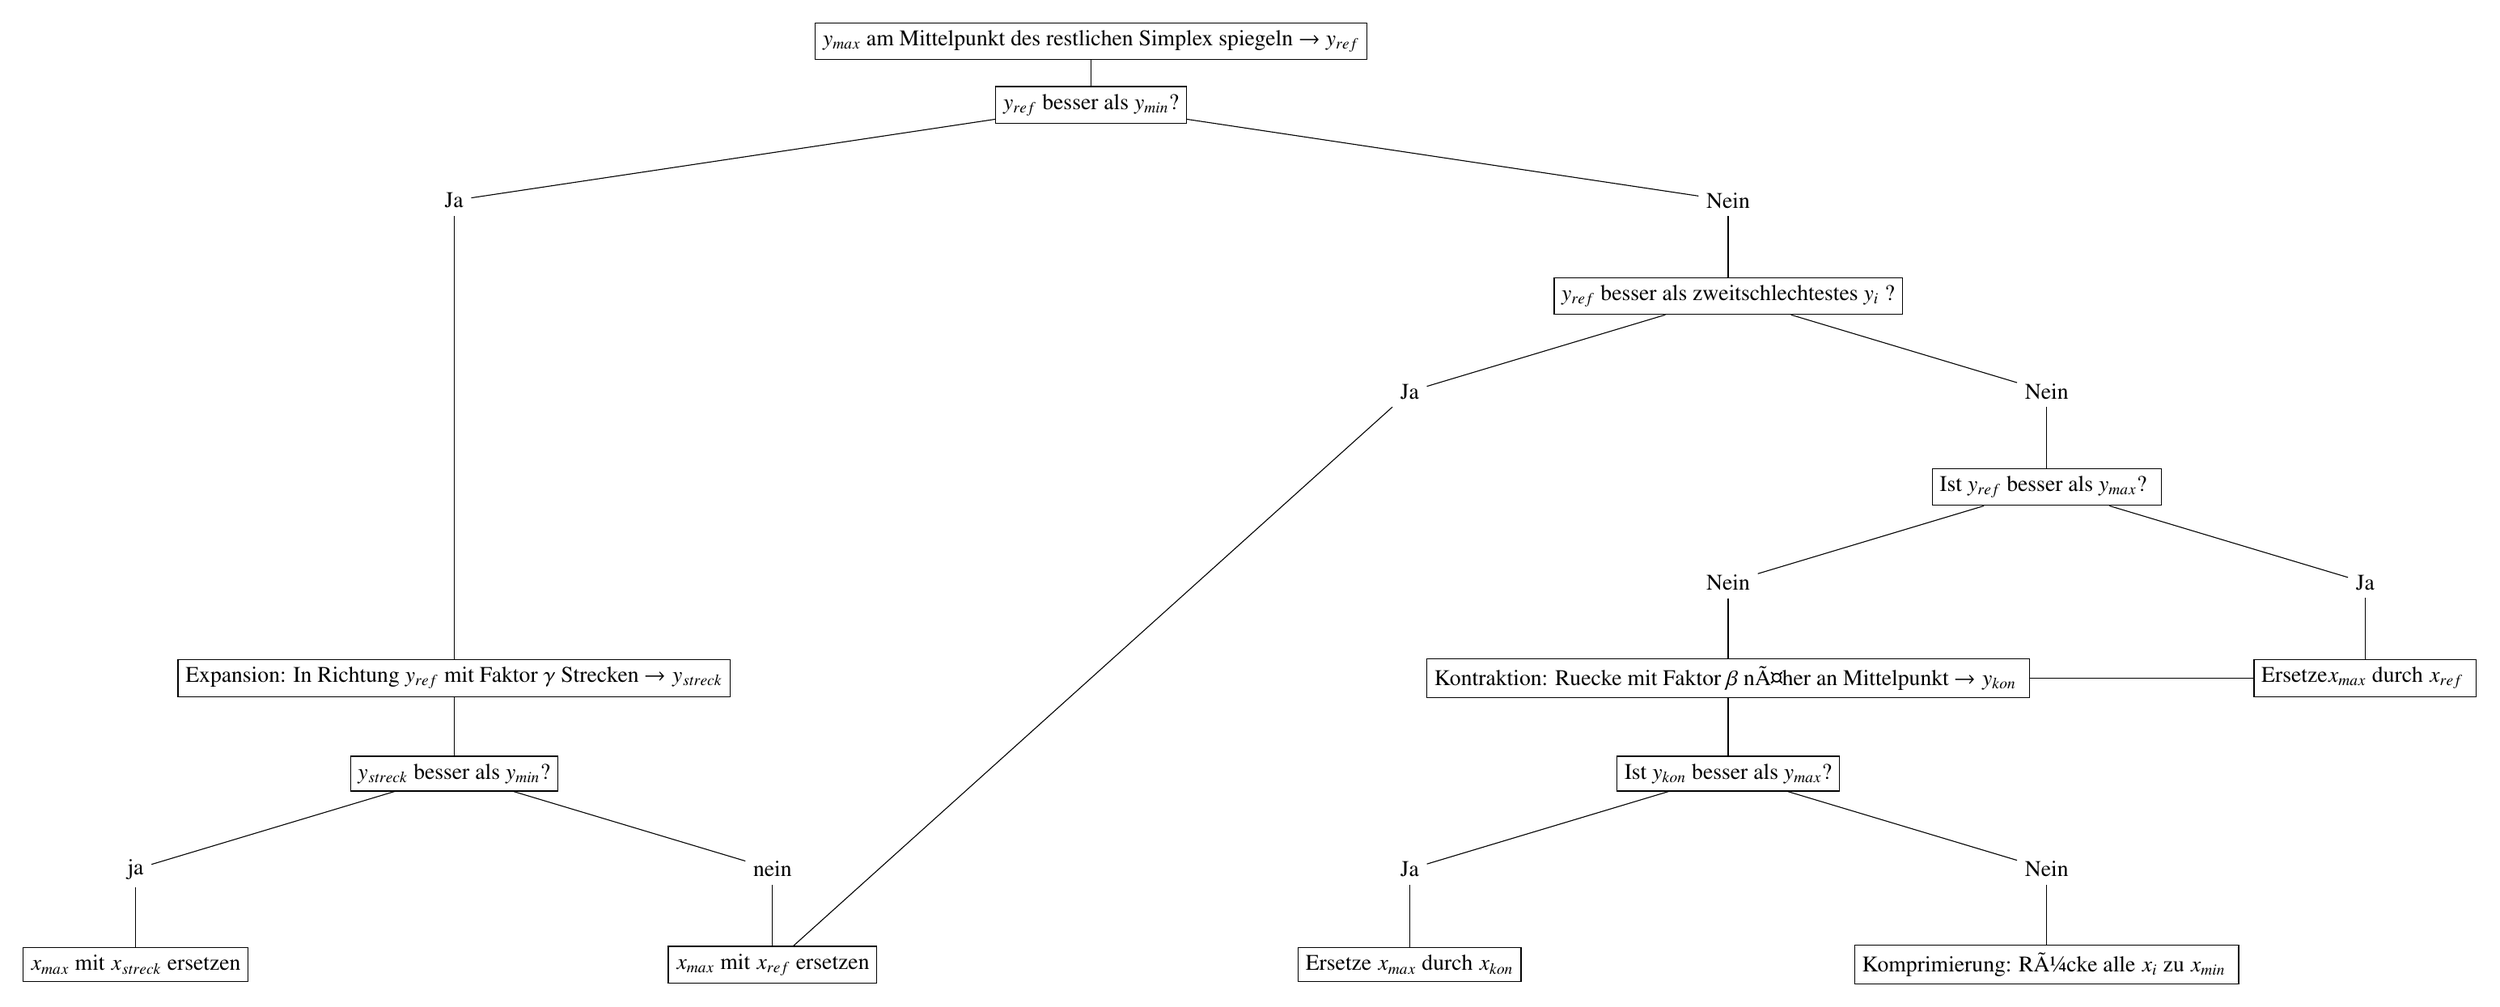
\begin{tikzpicture}[
  top/.style={draw,align=center},
  med/.style={draw,align=center},
  fin/.style={ellipse,draw,align=center}
]

\tikzstyle{level 1}=[sibling distance=200mm,align=center]
\tikzstyle{level 2}=[sibling distance=100mm,align=center]
%\tikzstyle{level 3}=[sibling distance=100mm]


\node (start) at (0,1)[draw] {$y_{max}$ am Mittelpunkt des restlichen Simplex spiegeln $\rightarrow$ $y_{ref}$};

\node[top](top){$y_{ref}$ besser als  $y_{min}$?}
	child { node {Ja} child {child { child  { child { child {
		node[med] {Expansion: In Richtung $y_{ref}$ mit Faktor $\gamma$ Strecken  $\rightarrow y_{streck} $}
		child{
			node[med]  {$y_{streck}$ besser als $y_{min}$?}
			child { node {ja}
			child { node [med]{$x_{max}$ mit $x_{streck}$ ersetzen} }}
			child { node {nein}
			child { node(a2) [med]{$x_{max}$ mit $x_{ref}$ ersetzen} }}
		}
	}}}}}}
	child {
		node {Nein}
		child  {
		node [med] {$y_{ref}$ besser als zweitschlechtestes $y_i$ ?}
		child { node (b1) [] {Ja} }
		child { node {Nein} 
		child { node[med] {Ist $y_{ref}$ besser als $y_{max}$? }
			child {node{Nein}
				child { node (kont)[med] {Kontraktion: Ruecke mit Faktor $\beta$ näher an Mittelpunkt $\rightarrow y_{kon}$ }
					child { node[med]  {Ist $y_{kon}$ besser als $y_{max}$?}
						child {node {Ja}
							child {node[med] {Ersetze $x_{max}$ durch $x_{kon}$}}
						}
						child {node {Nein}
							child {node[med] {Komprimierung:  Rücke alle $x_i$ zu $x_{min}$ } }
						}
					}
				}
			}
			child {node {Ja}
				child { node (zukont)[med] {Ersetze$ x_{max}$ durch $x_{ref}$ } }
			}
		}
		}
	}
	}
;
\draw (zukont) -- (kont);
\draw (b1) -- (a2);
\draw (start) --(top);

\end{tikzpicture}


\subsection{Probleme des Verfahrens}


\section{Beispiele}
Auf Grund seines eher einfachen Entscheidungsbaums ist es nicht sehr aufwendig den Algorithmus in einer entsprechenden Programmiersprache wie C zu implementieren. Eine Schleife mit den richtigen if-else-Abfragen und man hat einen funktionierenden Simplex-Downhill programmiert.\\
Nat"urlich ist der Algorithmus auch in Matlab integriert, man kann ihn mittels der Funktion \textbf{fminsearch} aufrufen. 
Der einfachste Aufruf erfolgt, indem man der Funktion \textbf{fminsearch} die Zielfunktion \textbf{fun} sowie den Startwert \textbf{$x_0$} "ubergibt. Wobei der R"uckgabewert ein neuen x-Wert ist, welcher den Funktionswert $fun(x)$ kleiner werden l"asst. 
\begin{lstlisting}
	x = fminsearch(fun,x0)
\end{lstlisting} 
Will man nun beispielsweise beobachten, wie der Algorithmus das Minima sucht, kann man folgenden Code verwenden: 
\begin{lstlisting}[style=Matlab]
%------------------------------------------------------------
%Initialisierung
%------------------------------------------------------------
xBorder = 10; 
teration = 20; 
x = (-xBorder:0.1:xBorder);     %Dimensionen x und y
y = (-xBorder:0.1:xBorder); 

[xx, yy] = meshgrid(x,y);       %meshgrid fuer spaetere Ausgabe
Fun = FUNKTION_SEINER_WAHL(xx,yy); %Berechne Funktionswerte

x_newFun = [4.9,4.9];           %Startwert
z_newFun = 0;                   %Funktionswert
x_Fun = zeros(2,2*teration+1);  %Vektor f"ur x1,x2
z_Fun = zeros(1,2*teration+1);  %Vektor f"ur Funktionswerte
options = struct('MaxIter',3);  %Einstellungen fminsearch
%------------------------------------------------------------
%Berechnung Simplex-Downhill
%------------------------------------------------------------
for i=1:(2*teration+1)
	[x_newFun z_newFun] = fminsearch(@FUNKTION_SEINER_WAHL,x_newFun,options2);
	x_Fun(1,i) = x_newFun(1,1);
	x_Fun(2,i) = x_newFun(1,2); 
	z_Fun(i)   = z_newFun; 
end
%------------------------------------------------------------
%Ausgabe Resultate
%------------------------------------------------------------
%Darstellung mittels H"ohenlinien
figure; 
contour(xx,yy,Fun,50);      %Zahl am Ende gibt an, wieviele 
                            %H"ohenlinien geplottet werden
hold on; 
for i=1:length(x_Fun)       %For-Schleife f"ur Visualisierung
    plot(x_Fun(1,i),x_Fun(2,i),'-*r'); 
    pause(0.5)              %Pause von 0.5 Sekunden
end
hold off; 

%Darstellung in 3D
figure; 
mesh(xx,yy,Fun);
hold on; 
plot3(x_Fun(1,:),x_Fun(2,:),z_Fun(:),'r','linewidth',4); 
hold off; 
grid on; 
\end{lstlisting}
Mittels dem in der Initialisierung definierten Struct kann man der Funktion einige Optionen "ubergeben. 
In diesem Fall wird dem Algorithmus mitgeteilt, wieviele Iterationen er pro Aufruf durchf"uhren soll. 
Wenn man - wie in unserem Fall - die Werte beobachten will, so sollte diese Zahl m"oglichst klein sein, darf jedoch nicht kleiner als 2 sein (warum auch immer).
Im folgenden wurde der Code auf die Himmelblau-Funktion angewendet: 
\begin{equation}
	f_{hb} = (x_1^2 + x_2 -11)^2 + (x_1+x_2^2-7)^2
\end{equation}
Diese Funktion hat 4 globale Minima: 
\begin{subequations}
	\begin{align}
		f(3,2) &= 0 \\
		f(-2.81,3.13) &= 0\\
		f(-3.78,-3.28) &= 0\\
		f(3.58,-1.85) &= 0
	\end{align}
\end{subequations}
Auf die Funktion wurden zwei Simplex los gelassen, je in gegen"uberliegenden Ecken (9,9) und (-9,-9).\\
Man sieht deutlich, dass beide Simplexe das ihnen n"achstgelegene Minima ansteuern. 
\begin{figure}[h]
	\centering
	\includegraphics[width=0.8\textwidth]{../bilder/HimmelblauHoehen.jpg}%
  	\caption{Simplexe auf Himmelblau-Funktion}%
	\label{fig:HB1}%
\end{figure}
\newpage
\begin{figure}[h]
	\centering
	\includegraphics[width=0.8\textwidth]{../bilder/Himmelblau3DRot.jpg}%
  	\caption{Rotes Simplex}%
	\label{fig:HB2}%
\end{figure}
\begin{figure}[h]
	\centering
	\includegraphics[width=0.8\textwidth]{../bilder/Himmelblau3DSchwarz.jpg}%
  	\caption{Schwarzes Simplex}%
	\label{fig:HB3}%
\end{figure}
\newpage
Beim folgenden Bild sieht man, wie der Algorithmus auf die Quadratfunktion angewendet wird, die interne Iterationszahl von \textbf{fminsearch} ist dabei auf 2 gesetzt und der Algorithmus wird 20 mal durchgef"uhrt.\\
In der Graphik sieht man, dass der Algorithmus eher langsam konvergiert, jedoch von beiden Seiten her dasselbe Resultat erzielt. 
\begin{figure}[h]
	\centering
	\includegraphics[width=0.8\textwidth]{../bilder/Quadrat.jpg}%
  	\caption{Simplex-Downhill auf Quadratfunktion angewendet}%
	\label{fig:SQ1}%
\end{figure}
\section{Variationen}
Es gibt verschiedenste Variationen des Downhill-Simplex Algorithmus.
Einige verwenden zusätzliche Freiheitsgrade, wie z.B. einen Parameter
$\sigma$, welcher $\beta$ bei Komprimierung ersetzt.

Auch gibt es Erweiterungen welche statistische Auswertung bei verrauschten Zielfunktionen (siehe \figref{fig:downhillRauschen1}) durchführen.
Verrauschte Zielfunktionen treten unter anderem auf wenn man Parameter f"ur ein System optimieren will, welche sich nur durch Messung vergleichen lassen.
Obwohl auch der ''normale`` Downhill-Simplex mehr oder weniger funktioniert (siehe \figref{fig:downhillRauschen2}), hat er m"uhe zu konvergieren, da er immer auch die Chance hat sich fälschlicherweise auszudehnen.
Wie man sieht ist viel Potential vorhanden indem der Einfluss des Rauschens verringert wird.
Informationen dazu unter \footnote{\url{http://www.informs-sim.org/wsc91papers/1991_0126.pdf}}
\begin{figure}[h]
\centering
\includegraphics[width=0.8\textwidth]{../bilder/HimmelblauRandom/himmelblauoverview.png}
\caption{Verrauschte Zielfunktion}
\label{fig:downhillRauschen1}
\end{figure}

\begin{figure}[h]
\centering
\includegraphics[width=0.8\textwidth]{../bilder/HimmelblauRandom/himmelblauall.png}
\caption{Beispiel Verlauf Simplex mit verrauschter Zielfunktion}
\label{fig:downhillRauschen2}
\end{figure}

\listoffigures
\begin{thebibliography}{widestlabel}
	%---------------------------------------------------------------------------------------------------
	%B�cher
	%---------------------------------------------------------------------------------------------------
	\bibitem[1]{bib:buch1}{Dr. Ludwig Fahrmeir,Dr. Alfred Hamerle,Dr. Gerhard Tutz, \textit{Multivariate statistische Verfahren},Verlag de Gruyter, 2 Auflage, 1996}

	\bibitem[2]{bib:buch2}{Dr. Lothar Harzheim, \textit{Strukturoptimierung: Grundlagen und Anwendungen}, Verlag Harri Deutsch, 2 Auflage, 2007}
	%---------------------------------------------------------------------------------------------------
	%Manuals/Datasheets
	%---------------------------------------------------------------------------------------------------
	\bibitem[3]{bib:link1}{ http://alphard.ethz.ch/, \textit{Erweiterung der Intervallunterteilungsmethoden Downhill Simplex}}

	\bibitem[4]{bib:link2}{http://en.wikipedia.org/, \textit{Nelder-Mead method}}

	\bibitem[5]{bib:link3}{http://de.wikipedia.org/, \textit{Downhill-Simplex-Verfahren}}
	
	\bibitem[6]{bib:link4}{http://de.wikipedia.org/, \textit{Simplex (Mathematik)}}

\end{thebibliography}


\end{document}
